\chapter{Metaheuristics}

\section{What is a metaheuristic?}
A metaheuristic is a problem-solving strategy that consists in a set of steps, a method to be short,
with the purpose of finding good solutions to optimization problems. Unlike heuristics, they are not dependent or 
tailored to a specific problem in particular, instead they are general problem-solving frameworks applicable
to a wide range of cases.\\
While heuristics are typically very specific on how we should operate when executing them, metaheuristics show a 
higher degree of abstraction, explaining the general approach that we should have, and leaving the actual details
of the implementation to the researcher.\\
They do not provide guarantees on the optimality of the solution returned, but they aim to find high-quality solutions
efficiently, this is why they often work in an iteratively manner, repeating a set of steps for a determined
amount of times, until some convergence factor is reached, or maybe until the solution found is considered good enough. 
This also explains the frequent presence of parameters to tune in this kind of methods. This difference with the heuristics 
can be confirmed also by the ones that we explored in this work. We can notice that the classic version of both 
\textit{nearest neighbor} and \textit{extra milage} do not involve any further step past the moment in which we 
reach a feasible solution, while on the metaheuristics that we will see we always start from an existing solution,
trying to improving it along the way.\\
Popular metaheuristics that we worked on are \textit{Simulated Annealing}, \textit{Genetic algorithm}, \textit{Tabu Search},
and \textit{Variable Neighborhood Search0}.


\section{2-Opt}
The 2-opt metaheuristic is a local search method used to improve the solution in optimization problems. It is based on the
idea of iteratively improving a feasible solution of the problem by swapping pairs of edges creating a new solution. The name
comes from the fact that it works on two different edges of the graph at a time.\\
The method works on an existing solution of the problem, in an iteration of 2-opt two edges are removed from the tour, and replaced
by new edges, that reconnect the tour but in a reverse way.\\

\begin{figure}
    \centering
    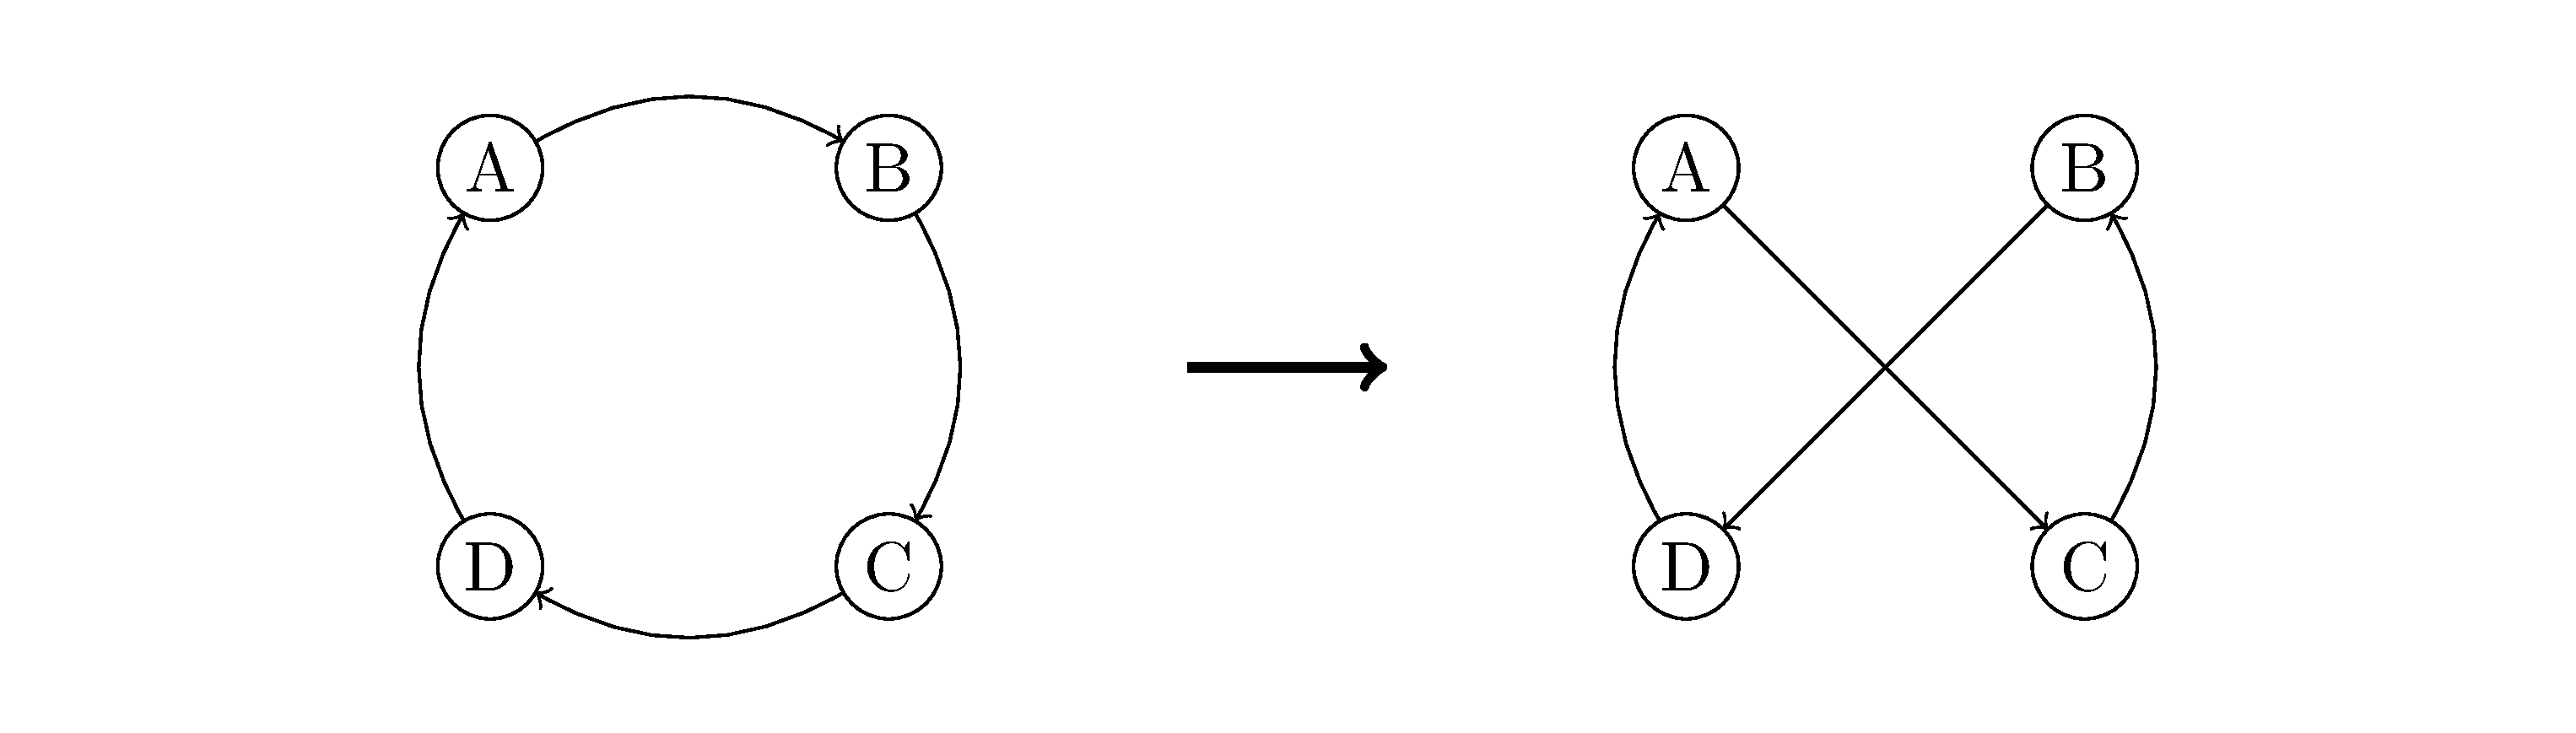
\includegraphics{2opt_1.png}
    \caption{2-opt iteration}
    \label{fig:2-opt}
\end{figure}

Once the edges are swapped the total cost of the tour is recalculated, and if it is lower than the previous cost, the swap is 
integrated in the solution permanently, or until a better swap involving one of those two edges is found.\\
This operation is iterated across all possible pairs of the tour, and is repeated until a time limit is reached, or 
no further improvements are possible (which involves checking all possible combinations many time, making it infeasible for 
real-life complex scenarios).\\
2-opt can improve significantly a solution, while maintaining an acceptable computational complexity across the board. Its
main limitation is the fact that due of it being a local search method, it may get stuck in local optima and fail to find the
global optima.

\subsection{Implementation}
In our implementation of 2-opt we decided to optimize heavily the method using AVX functions rather than multithreading 
(NOTE: check, and why AVX).
The function that takes care of the application of the metaheuristic is apply2OptBestFix, to which we pass the solution to refine, 
and will apply the options selected at launch. 
The heart of the algorithm lies in the two specular functions _2OptBestFix and _2OptBestFixApprox.
The former will compute the exact edge cost when evaluating edge swaps, considering the actual distance between the points and delivering 
a more precise result, with the cost of a slower computation, especially for larger instances.
The latter uses an approximated computation of the edges cost and provides a faster iteration time, with the counterpart of possibly 
producing slightly worse solutions. 
These two methods will iterate over all possible pairs of edges in the tour and compute the potential decrease in total tour length if 
we were to apply the swap.
The data regarding the best swap found so far, offset of the cost and the edges, is kept in the bestFix struct, to which we will compare 
each potential swap and which will be then implemented at the end of the iteration.


\subsection{3-Opt}
The 3-opt metaheuristic is an extension of 2-opt, with the difference that it no longer considers two-edge combinations but three-edge
combinations instead. This allows for a larger neighborhood of solutions, and opens to the possibility of escaping situations of local minima
that 2-opt might not able to avoid. It is worth mentioning that while the neighborhood of solutions is larger, escaping from all
local minima is not garanteed and generally not possible with this method.\\
The process is mechanically the same as for 2-opt. As shown in figure \ref{fig:3-opt}, starting from an existing solution, we iteratively 
consider three edges instead oftwo, and we change the way they are connected, looking for the one that has lower total cost. If a combination 
is found to improve the total cost of the solution then the swap is implemented, otherwise a different set of three edges is taken into consideration.
Just as for 2-opt this iterative process can continue until a time limit is reached or until no more improving moves are possible.

\begin{figure}
    \centering
    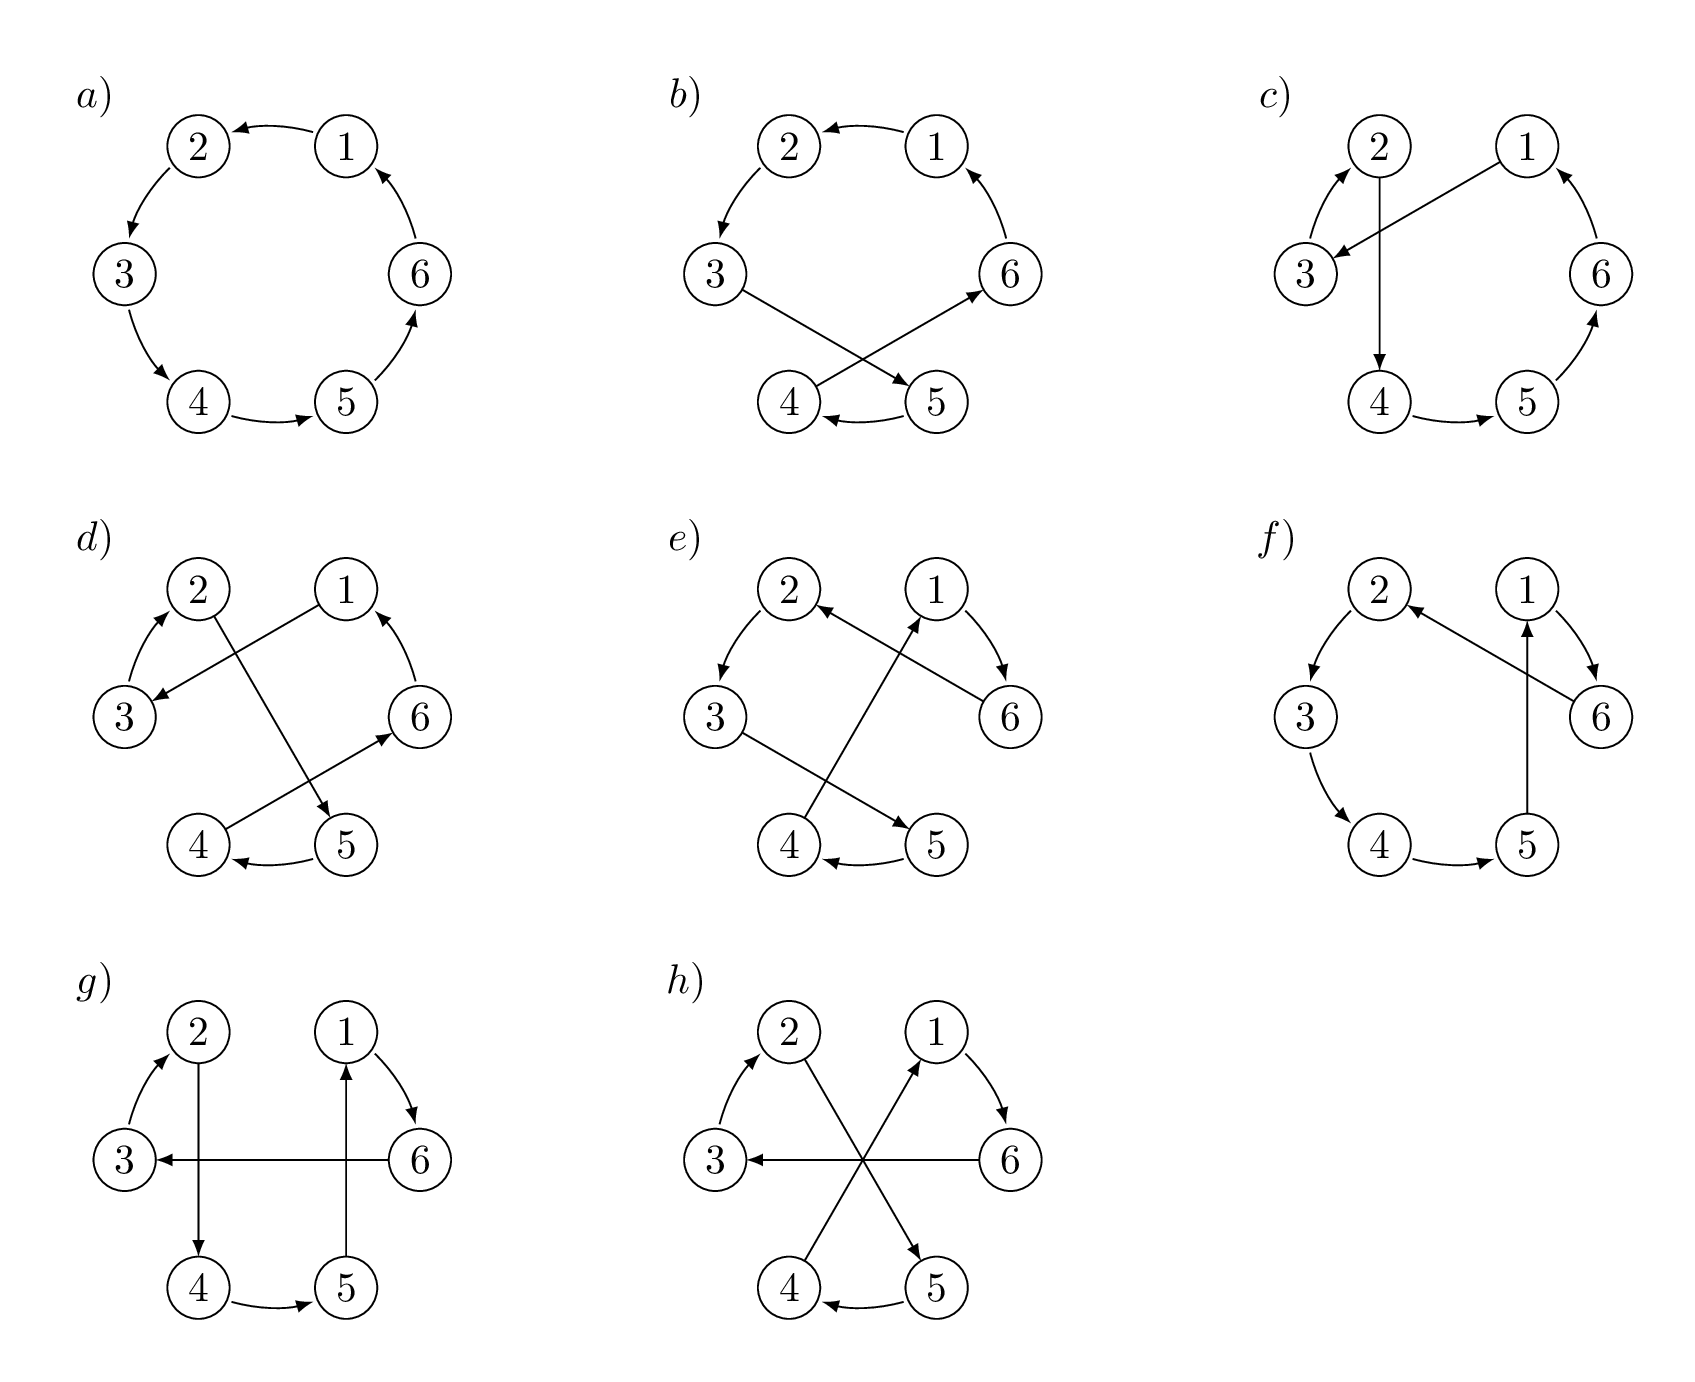
\includegraphics[width=1\textwidth]{3opt_1.png}
    \caption{3-opt computation. As can be observed, not all swaps are implemented in the solution, but only the ones that improve its cost.}
    \label{fig:3-opt}
\end{figure}

\section{Tabu Search}
Tabu search is a metaheuristic that focuses on escaping local minima. The idea is to avoid solutions that we know that cannot lead
to the global optima.\\
Let's assume that we alredy have a refined solution, and that we have reached a local minima, let's call this solution $x_k$. 
Trying to further refine it using 2-opt will not provide any improvement, since it is a method that is not designed to escape this
kind of situations. Hence, the only way to move from this neighborhood of solutions is to accept a \textit{bad} move, in other words
we need to perform a swap of some edges that will worsen the solution, generating a new one called $x_{k+1}$, in the hope from it we will be 
able to reach a better one.\\
The way that Tabu Search does this is by implementing a list of edges that cannot be touched, called \textit{tabu list}. Any of the
edges in this list are \textit{fixed} and we are not allowed to move them with a 2-opt-type move, which forbids a backwards movement
from $x_{k+1}$ to $x_k$. Logically, without this list, if we were to perform a swap that worsens the solution and we were to 
apply 2-opt right after we would just go back to $x_k$, which is the local minima we are trying to escape from.\\
Intuitively the size of the list has to be limited, otherwise we could run into the issue of blocking too many edges and we would not
be able to perfom any move. This size is called \textit{tenure}, and could be a fixed amount or it could be adaptive depending on the
instance of the problem we are approaching. When the list is full, we start replacing the edges in it starting from the older ones.
As the other metaheuristic presented, this process can continue until a time limit or a certain number of iterations is reached, or
until the solution is considered good enough.

\subsection{Implementation}
TabuSearch is the main method that manages the execution of the tabu algorithm. After receiving the solution, it sets the tenure size, 
which is implemented as an array of struct Edge, accordingly to input. We implemented a check on the value passed for this parameter: if 
we don't receive any specific size the default value of 2 is set; if we receive a value that is larger of equal to the amount of nodes in 
the instace an error is thrown, since this will lead to the algorithm getting stuck; and lastly, if the value is larger than the 97\% of the 
number of nodes a warning message will indicate the possibility of the method getting stuck and not respecting the time limit.
After this, the function runTabu is launched whithin the threads and takes care of the execution of the metaheuristic, starting from the 
current best solution (CHECK IF ITS THE PASSED SOLUTION). The main loop that keeps going until the time limit consists in selecting two random 
edges in the solution, swapping them and locking one of the two by inserting it into the tenure. Once we have done that 2-opt is launched to 
refine the solution, and we keep relaunching it until there are no further improving moves possible, freeing the oldest element in the tenure 
before relaunching it every time. A counter is implemented to keep track of the number of iteration in which the method does not find a solution 
that is better than the best one found so far, and when it reaches a threshold the working solution of the thread is resetted back to the best one.


\section{Variable Neighborhood Search}
Variable Neighborhood Search (VNS) is a technique used to explore different neighborhoods of the solution space in order to find the
optimal solution of a problem. The idea is to, starting from a feasible solution, completely explore its neighborhood, and finding the
best solution in that neighborhood. After that we move onto another neighborhood and we explore that one. While we do this process
we keep track of the best solution found so far, and we replace it when a new neighborhood reveals a better minima.\\
In TSP, to explore the neighborhood of a solution we can use local search algorithms like 2-opt and 3-opt, while to change the neighborhood
we perform a swap on a higher amout of edges, five, for instance. Doing this allows us change the space in which we search for the 
solution using local search maintaining most of the existing tour untouched.\\

\begin{figure}
    \centering
    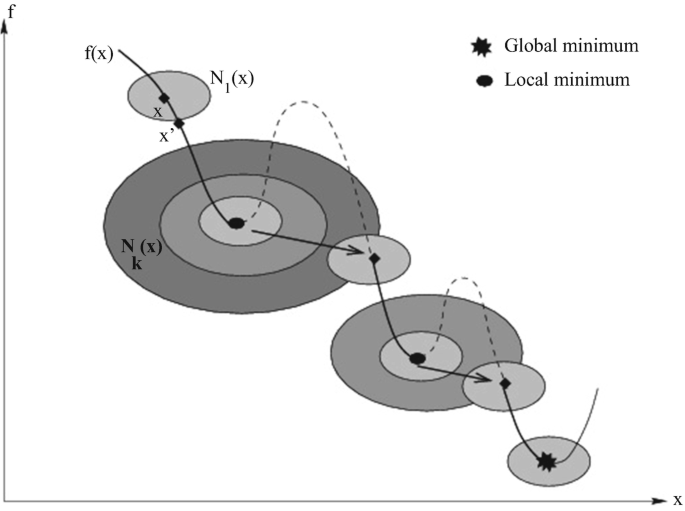
\includegraphics[width=1\textwidth]{vns_1.png}
    \caption{Iteration process of VNS}
    \label{fig:vns}
\end{figure}

VNS balances exploration (through varying neighborhood structures) and exploitation (through local search) to efficiently search the solution space.
The number of edges that we decide to swap can be dependent of the size of the instance, if we were working on a small instance, e.g. 
~50 nodes, swapping more than ten edges could result in a change way too big of the starting solution, worsening it unnecessarily.

\subsection{Implementation}
For the implementation of VNS we have the main function VariableNeighborhoodSearch which is in charge of managing the various threads initialization 
and coordination, along with the time management in order to maintain the execution of the algorithm within the time limit provided in input.
Inside the threads we will run parallely the function runVns, which performs the actual algorithm.
The loop inside the threads will start by taking the passed solution and perform a repeating cycle of 2-opt operations and kicks. 2-opt is in charge 
of searching the local space of the solution, while the kick will ensure a traslation to a neighboring search space.
For the kick we implemented a swap of a dynamically chosen amount of edges. We did this to adapt to different scales of instances, since a fixed 
amount of edges swaps (e.g. five each time) could result in a non-effective enough of a neighborhood change for large instances. All the edges involved in the kick are selected randomly.
After each execution of 2-opt the obtained solution will be compared with the saved best solution found so far, and, if the cost is improved, the 
best solution gets updated. Note that the best solution is shared among the threads and its access is managed by mutex.

\section{Simulated Annealing}
Simulated Annealing (SA) is a probabilistic metaheuristic inspired by the annealing process in metallurgy, where a material in heated
and then slowly cooled in order to improve its quality. The main parameter for this method is in fact called \textit{temperature}.
The value of this parameter indicates the probaility for which we allow our method to accept bad moves (e.g. swap two edges that 
don't improve the solution cost). Initially this parameter is set high, which allows for a greater exploration of the solution space.
At every iteration this parameter is scaled down (by a factor of $0.9$ or $0.95$ for example), gradually allowing for less and less 
bad moves, restricting the search space. 

\begin{figure}
    \centering
    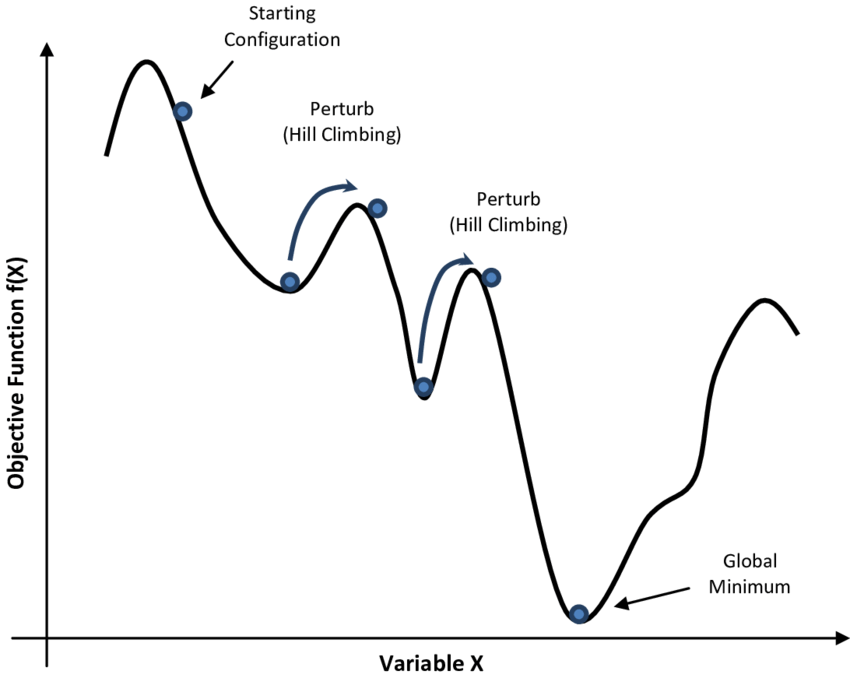
\includegraphics[width=1\textwidth]{sa_1.png}
    \caption{Iteration process of Simulated Annealing}
    \label{fig:sa}
\end{figure}

\subsection{Implementation}
For the implementation of Simulated Annealing we decided to set up a number of constants in order to be able to tweak the parameters of the 
method in input. Fixed parameters can work fine for instances of similar magnitude, but to allow for a good execution for both large and small 
instances we thought this was the best approach. The parameteres we are talking are:

\begin{enumerate}
    \item SAME_TEMP_MOVES_THRESHOLD: Number of moves to perform before reducing the temperature.
    \item TEMPERATURE_MULTIPLIER: Factor by which the temperature is multiplied to decrease it; should be slightly less than 1.
    \item STOP_TEMP: Temperature at which SA stops and runs a 2-opt algorithm for further optimization.
    \item MAX_TRIES_FUNC(n): Function to determine the maximum number of move attempts before increasing the temperature.
    \item USE_RATIO_ACCEPTANCE: A macro to toggle the use of ratio-based acceptance criteria.
\end{enumerate}


The execution of this metaheuristic is managed by the function SimulatedAnnealing, that mainly sets up the desired number of threads and launches them 
on the function runSimulatedAnnealing. 
The actual algorithm is then executed parallely within each thread until the time limit is reached. During this time we perform moves up to what we 
specified on STOP_TEMP, then we will launch the 2-opt metaheuristic to further refine the solution within its space. 
After a certain amount of non-improving iterations, we restart the method from the best solution found so far, which we are keeping track at all 
times and is accessible by the use of a mutex by all threads. This is to fully use the time provided in the time limit, and to give the method more chances to escape a local minima.


\section{Genetic}
\subsection{Implementation}
In a similar fashion of the algorithms previously presented, for the Genetic Algorithm we also have a main method, GeneticAlgorithm, that is in 
charge of managing the creation and synchronization of the various threads. The actual algorithm is performed then within each thread by the function runGenetic.
A series macros are used throughout the code to configure the genetic algorithm's behavior without hardcoding values. For example, the population 
size and the number of genetic operations (crossover, mutation, reintroduction) are dynamically calculated based on the instance parameters using 
POPULATION_SIZE, CROSSOVER_AMOUNT, MUTATION_AMOUNT and REINTRO_AMOUNT. 